%\documentclass[11pt]{report}
%\linespread{1.3} %1.3 for one and a half spacing, 1.6 for double
%\usepackage{amsmath, amsthm, amssymb, float, graphicx, caption, subcaption, cite, braket, url,color}
%%\usepackage[nohug,heads=vee]{diagrams}
%%\diagramstyle[labelstyle=\scriptstyle]
%%\graphicspath{{./Figures/}}
%\usepackage[margin=2.5cm]{geometry}
%%\title{Title}
%%\author{Chrysoula Vlachou}
%%\date{}
%\newtheorem{lemma}{Lemma}
%\newtheorem{theorem}{Theorem}
%\newtheorem{proposition}{Proposition}
%%\theoremstyle{definition}
%\newtheorem{definition}{Definition}
%\newcommand{\N}{\mathbb N}
%\newcommand{\R}{\mathbb R}
%\newcommand{\C}{\mathbb C}
%\newcommand{\Hilb}{\mathcal H}
%\newcommand{\HRule}{\rule{\linewidth}{0.5mm}}
%\newcommand{\mmobh}{\textlatin{M\"ob}(\mathbb{H})}
%\newcommand{\areah}{\textlatin{area}_{\mathbb{H}}}
%\newcommand{\dth}{d_{\mathbb{H}}}
%\newcommand{\tdth}{$d_{\mathbb{H}}$ }
%\def\h{\mathbb H}
%\DeclareMathOperator{\tr}{Tr}
%\def\I{\hat I}
%\def\ds{\displaystyle}
%\def\ppmod{\!\!\!\!\!\pmod}
%\newcommand{\q}[1]{\vec{#1}\cdot\vec{\sigma}}
%
%
%
%\newcommand{\innerproduct}[2]{\langle #1 | #2 \rangle}
%\def\mobh{\textlatin{M\"ob}({\mathbb H})}
%
%
%
%\begin{document}


\begin{center}
\begin{Huge}
\textbf{Part II\\ \vspace{\baselineskip}Phase Transitions of Topological Systems at Finite Temperature}\end{Huge}
\end{center}
\newpage


\chapter{Fidelity and Uhlmann connection analysis of fermionic systems undergoing phase transitions}

In this chapter, we analyse the behaviour of the fidelity and the Uhlmann connection with respect to thermal states in fermionic systems undergoing PTs. To this end, we will consider the space consisting of the parameters of the Hamiltonian and the temperature, as it provides a physically sensible base space for the principal bundle, describing the amplitudes of the density operator.

The chapter is organised as follows: in Section~\ref{sec:topo}, we perform the fidelity and Uhlmann connection analysis of PTs for paradigmatic models of 1D topologically non-trivial insulators (TIs) and superconductors (TSCs). We further confirm these results in Section~\ref{sec:edge}, by studying the behaviour of the edge states in these systems. In Section~\ref{sec:bcs} we investigate the behaviour of the fidelity and the Uhlmann connection in the case of a topologically trivial superconductor in 3D, as described by the BCS theory. We compare these results to the respective ones obtained in Section~\ref{sec:topo} and explain the reasons behind the different behaviours. In Section~\ref{sec:space}, we comment on the relevance of the choice of the base space in the study of PTs for topological systems.  In the last section, we summarise our results, present our conclusions and point out some possible directions of future work.


\vfill

\begin{center}
 *The work presented in this chapter corresponds to the work published in~\cite{mer:vla:pau:vie:17}.
\end{center}

\newpage




\section{Fidelity and $\Delta$ analysis of topological insulators and superconductors}
\label{sec:topo}
In our analysis we probe the fidelity and the quantity $\Delta$ associated to the Uhlamnn factor, as presented in Section~1.6 of the introductory Chapter 1, with respect to the parameters of the Hamiltonian describing the system and the temperature, independently. In this section, we will perform this study for paradigmatic models of TIs, namely the Su-Schrieffer-Heeger (SSH)~\cite{su:sch:hee:79} and the Creutz ladder~\cite{cre:99,ber:pat:ami:del:09} models, and TSCs, namely the Kitaev Chain~\cite{kit:cha:01} model in 1D. \\
These are free-fermion models, which can be described by quadratic Hamiltonians of the form
\begin{equation}
\mathcal{H}=\sum_{k\in\mathcal{B}}\Psi_k^\dagger H_k \Psi_k,
\end{equation}
where $\Psi_k^\dagger,\Psi_k$ are the Nambu spinors, constructed by the corresponding fermion creation and annihilation operators, depending on the specific model (insulator or superconductor) and $H_k$ is the single-particle Hamiltonian in momentum space. Notice that the sum is over all momenta in the first Brillouin zone $\mathcal{B}$. The single-particle Hamiltonians $H_k$ are of the form
\begin{equation}
H_k=E_k\ \vec{n}_k\cdot\vec{\sigma},
\end{equation}
where $E_k$ is the spectrum of $H_k$ that gives the band gap, $\vec{n}_k$ is the so-called winding vector pointing along the quantisation axis and $\vec{\sigma}=(\sigma_x,\sigma_y,\sigma_z)$ is the Pauli vector. Note that the symmetries that the Hamiltonians of topological systems possess, which we mentioned in the Introduction (TRS, PHS and CS), are imposed on the level of the single-particle $H_k$.\\
For our study, we analytically calculated the closed expressions for the fidelity and $\Delta$, with respect to thermal states $\rho=e^{-\beta \mathcal{H}}/Z$, where $\beta$ is the inverse temperature.  We used natural units $\hbar=k_{\text{B}}=1$, and we obtained

\begin{equation}
F(\rho,\rho')=\prod_{k\in\mathcal{B}}\frac{2+\sqrt{2\left(1+\cosh(E_k/2T)\cosh(E'_k/2T')+\sinh(E_k/2T)\sinh(E'_k/2T')\vec{n}_k\cdot\vec{n}'_k\right)}}{\sqrt{(2+ 2\cosh (E_k/2T))(2+2\cosh (E'_k/2T'))}},
\end{equation}
and 
\begin{equation}
\Delta(\rho,\rho')=F(\rho,\rho')-\prod_{k\in \mathcal{B}}\frac{2+2\left(\cosh(E_k/4T)\cosh(E'_k/4T')+\sinh(E_k/4T)\sinh(E'_k/4T')\vec{n}_k\cdot\vec{n}'_k\right)}{\sqrt{(2+ 2\cosh (E_k/2T))(2+2\cosh (E'_k/2T'))}}.
\end{equation}
For the details of the derivation, see Appendix A.

The Hamiltonian for the TI SSH model~\cite{su:sch:hee:79} is given by
\begin{equation}
\mathcal{H}=\sum_{i\in\mathbb{Z}}v c^{\dagger}_{i,A}c_{i,B}+w c^{\dagger}_{i,B}c_{i+1,A}+\text{H.c.},
\end{equation}
where $c_i$ are fermionic annihilation operators, $A,B$ correspond to the two parts of the dimerised chain and $v,w$ are coupling constants. The change of the difference $|v-w|$ between the two parameters of the Hamiltonian drives the topological PT. In particular, the PT occurs for $|v-w|=0$. Given two close points $(|v-w|,T)$ and $(|v-w|',T')=(|v-w|+\delta |v-w|, T+\delta T)$, we compute $F(\rho,\rho')$ and $\Delta(\rho,\rho')$ between the states $\rho=\rho(|v-w|,T)$ and $\rho'=\rho(|v-w|',T')$. To distinguish the contributions due to the change of Hamiltonian's parameter and the temperature, we consider the cases $\delta T = 0$ and $\delta |v-w| = 0$, respectively, see Figure~\ref{fig:fid:ssh}.

\begin{figure}[h!]
\begin{minipage}{0.33\textwidth}
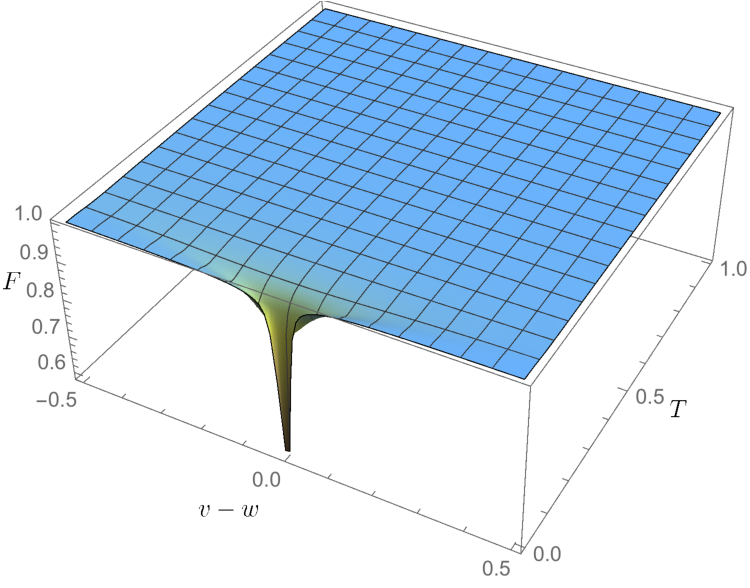
\includegraphics[width=0.7\textwidth,height=0.5\textwidth]{SSH_fidelity_theta.pdf}
\end{minipage}%
\begin{minipage}{0.33\textwidth}
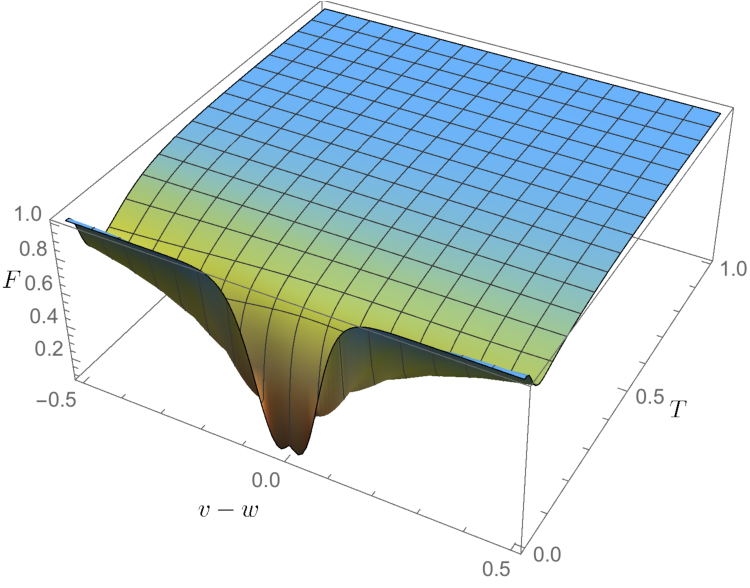
\includegraphics[width=0.7\textwidth,height=0.5\textwidth]{SSH_fidelity_T.pdf}
\end{minipage}
\begin{minipage}{0.33\textwidth}
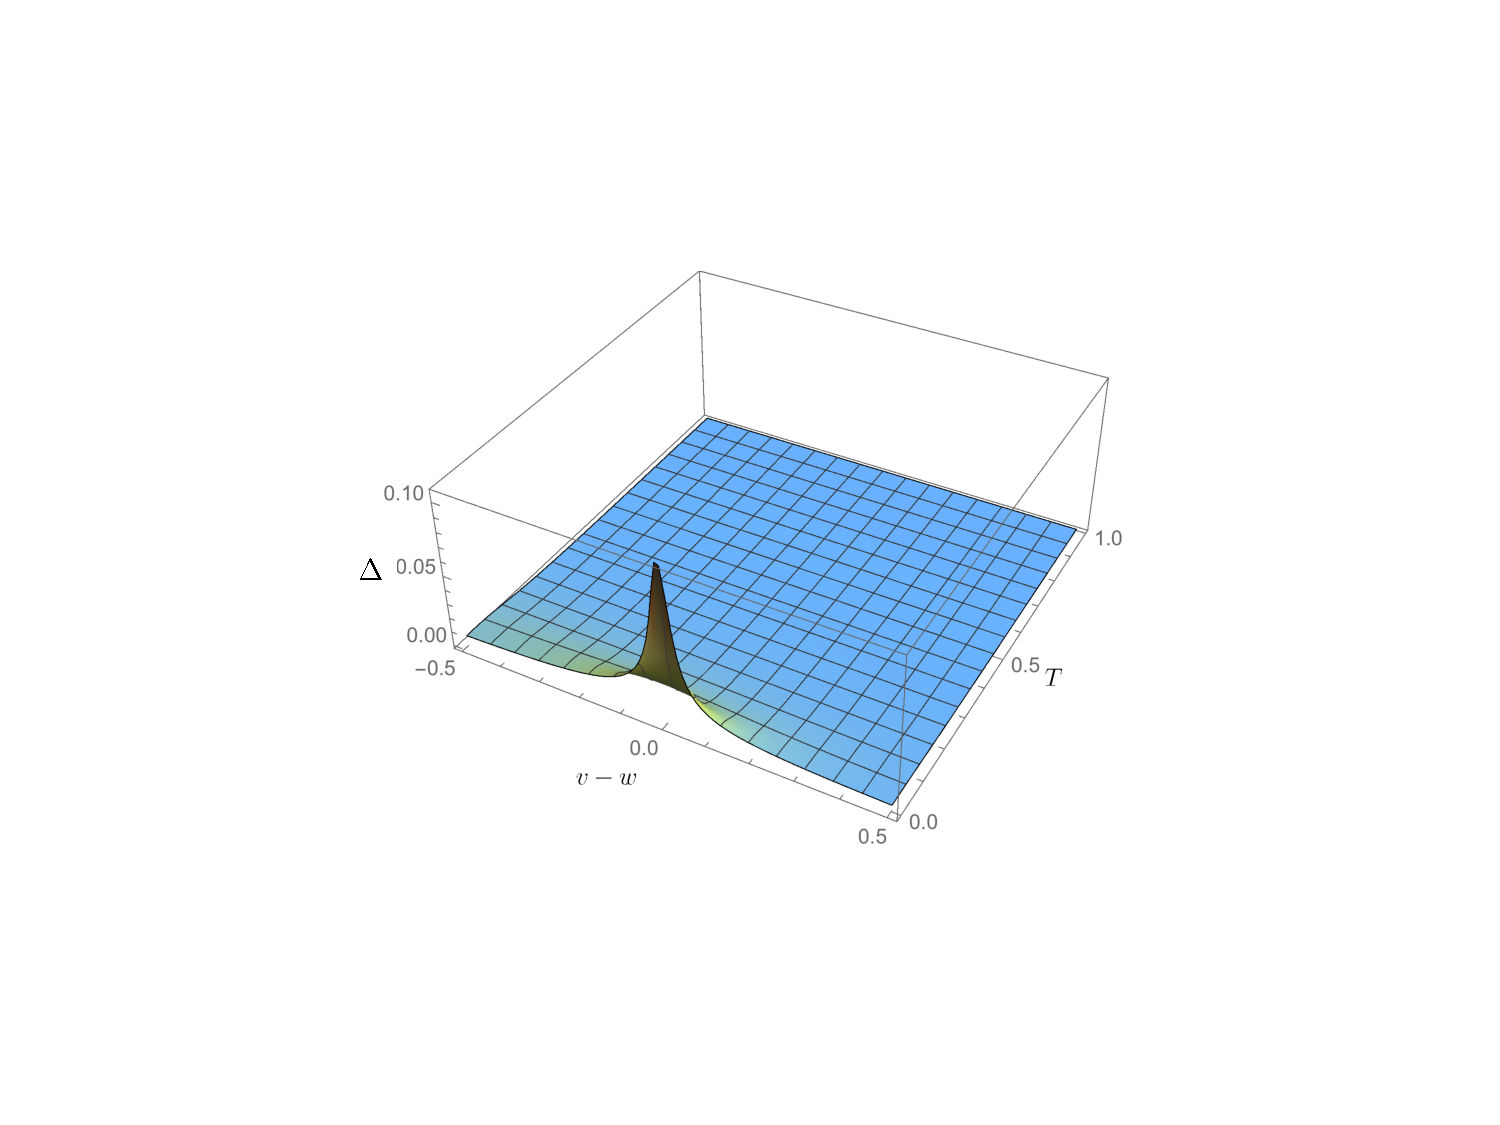
\includegraphics[width=0.7\textwidth,height=0.5\textwidth]{SSH_uhlmann_theta.pdf}
\end{minipage}%
\caption{The fidelity for thermal states $\rho$, when probing the parameter of the Hamiltonian that drives the topological PT $\delta |v-w| =|v-w|'-|v-w|=0.01$ (left), and the temperature $\delta T=T'-T=0.01$ (centre), and the Uhlmann connection, when probing the parameter of the Hamiltonian $|v-w|$ (right), for the TI SSH model (representative of the symmetry class BDI). The plot for $\Delta$ when $\delta |v-w|=0$ is omitted, since it is equal to zero everywhere.}
\label{fig:fid:ssh}
\end{figure}
The Hamiltonian for the TI Creutz Ladder model~\cite{cre:99,ber:pat:ami:del:09} is given by
\begin{eqnarray}
\mathcal{H}=& -\sum_{i\in\mathbb{Z}}K\left(e^{-i\phi}a_{i+1}^{\dagger}a_{i}+e^{i\phi}b_{i+1}^{\dagger}b_{i}\right)\nonumber\\
&+K(b_{i+1}^{\dagger}a_{i}+a_{i+1}^{\dagger}b_{i})+Ma_{i}^\dagger b_i +\text{H.c.},	
\end{eqnarray}
where $a_i,b_i$, with $i\in\mathbb{Z}$, are fermion annihilation operators, $K$ and $M$ are hopping amplitudes (horizontal/diagonal and vertical, respectively) and $e^{i\phi}$ is a phase factor associated to a discrete gauge field. We take $2K=1$, $\phi=\pi/2$. Under these conditions, the system is topologically nontrivial when $M<1$ and trivial when $M>1$. 
Similarly to the case of the SSH model, for two close points $(M,T)$ and $(M',T')=(M+\delta M, T+\delta T)$, we compute $F(\rho,\rho')$ and $\Delta(\rho,\rho')$ between $\rho=\rho(M,T)$ and $\rho'=\rho(M',T')$ and we consider the cases $\delta T = 0$ and $\delta M = 0$, respectively, see Figure~\ref{fig:fid:cl}.




\begin{figure}[h!]
\begin{minipage}{0.32\textwidth}
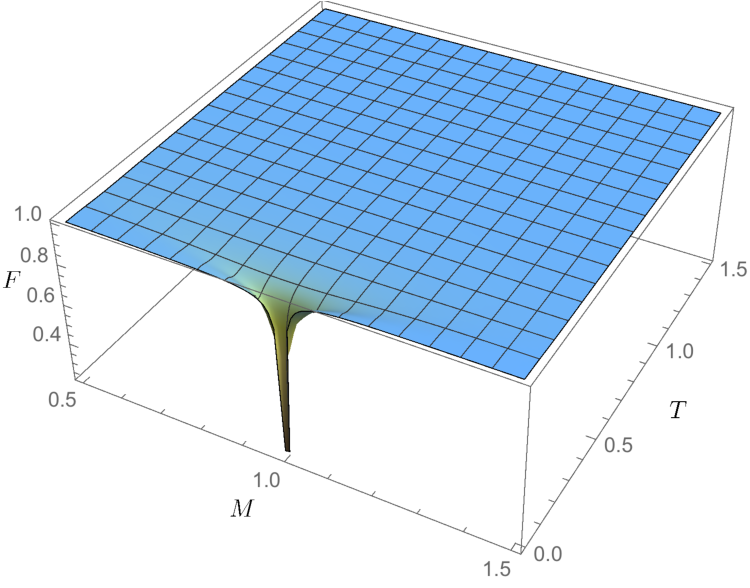
\includegraphics[width=0.7\textwidth,height=0.6\textwidth]{CL_fidelity_theta.pdf}
\end{minipage}
\begin{minipage}{0.32\textwidth}
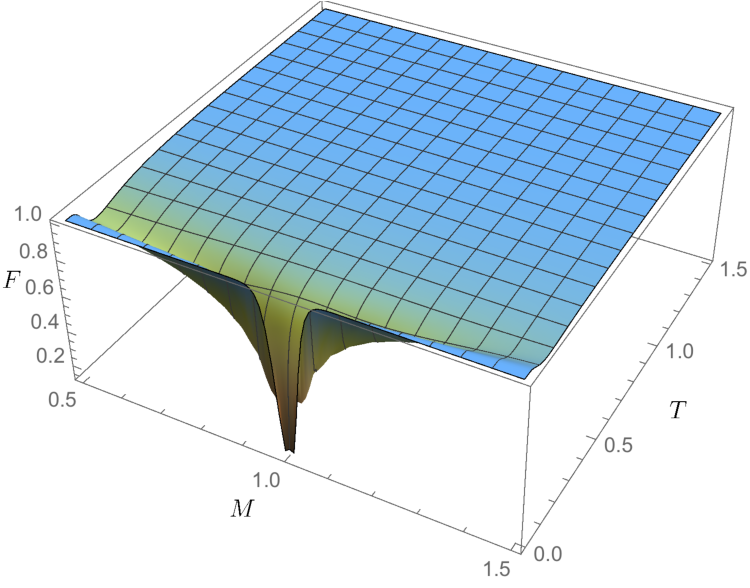
\includegraphics[width=0.7\textwidth,height=0.6\textwidth]{CL_fidelity_T.pdf}
\end{minipage}
\begin{minipage}{0.32\textwidth}
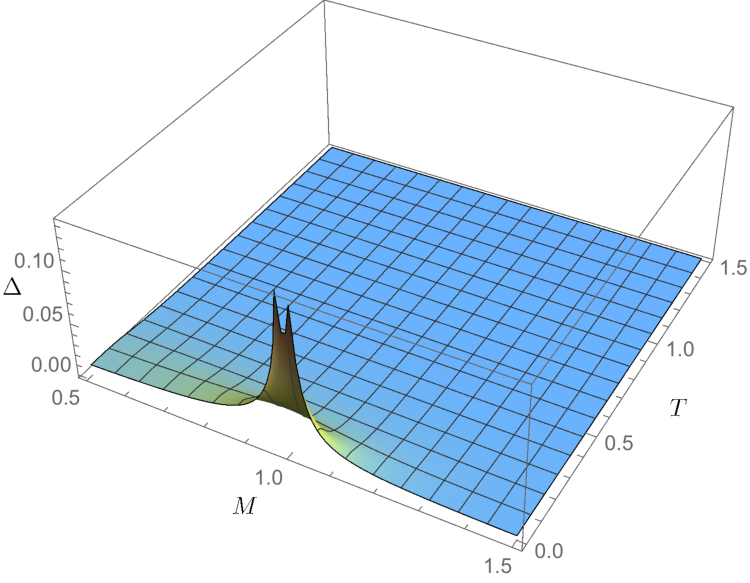
\includegraphics[width=0.7\textwidth,height=0.6\textwidth]{CL_uhlmann_theta.pdf}
\end{minipage}
\caption{The fidelity for thermal states $\rho$, when probing the parameter of the Hamiltonian that drives the topological PT $\delta M =M'-M=0.01$ (left), and the temperature $\delta T=T'-T=0.01$ (centre), and the Uhlmann connection, when probing the parameter of the Hamiltonian $M$ (right), for the TI Creutz ladder model (representative of the symmetry class AIII). The plot for $\Delta$ when deforming the thermal state along $T$ is omitted since it is equal to zero everywhere.}
\label{fig:fid:cl}
\end{figure}

Finally, we present our quantitative results for the TSC model. The Hamiltonian for the Kitaev Chain model~\cite{kit:cha:01} is given by
\begin{equation}
\mathcal{H}=-\mu\sum_{i=1}^N c^{\dagger}_i c_i+\sum_{i=1}^{N-1}\left[-t(c^{\dagger}_{i+1}c_i+c^{\dagger}_ic_{i+1})-|\Delta|(c_ic_{i+1}+c^{\dagger}_{i+1}c^{\dagger}_i)\right],
\end{equation}
 where $\mu$ is the chemical potential, $t$ is the hopping amplitude and $\Delta$ is the superconducting gap. 
 We fix $t=0.5,\Delta=1$, while the change of $\mu$ along the sites of the line drives the topological PT. In particular, the PT occurs at $\mu=1$ (gap closing point). Again, we calculate $F(\rho,\rho')$ and $\Delta(\rho,\rho')$ for $\rho=\rho(\mu,T)$ and $\rho'=\rho(\mu',T')$ for two close points $(\mu,T)$ and $(\mu',T')=(\mu+\delta \mu, T+\delta T)$ of the parameter space. In Figure~\ref{fig:fid:kit}, we show our results when probing the parameter of the Hamiltonian ($\delta T = 0$) and the temperature ($\delta \mu = 0$), separately.
  
 \begin{figure}[h!]
\begin{minipage}{0.33\textwidth}
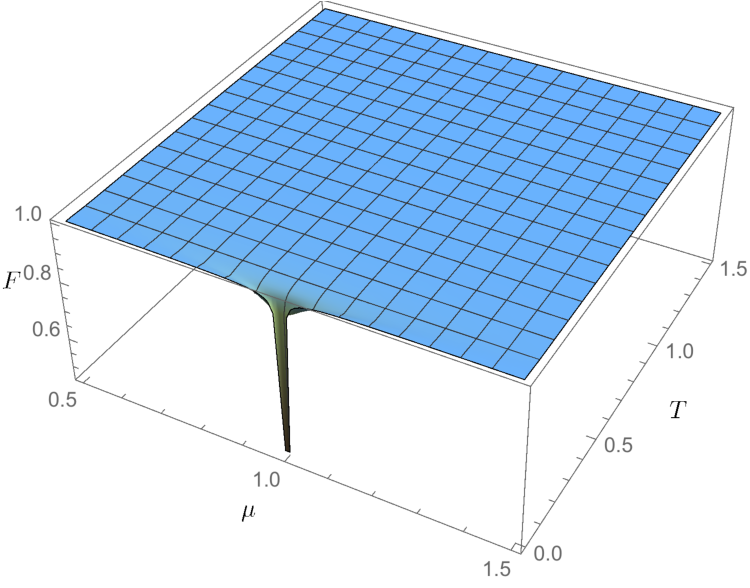
\includegraphics[width=0.7\textwidth,height=0.5\textwidth]{kitaev_fidelity_theta.pdf}
\end{minipage}%
\begin{minipage}{0.33\textwidth}
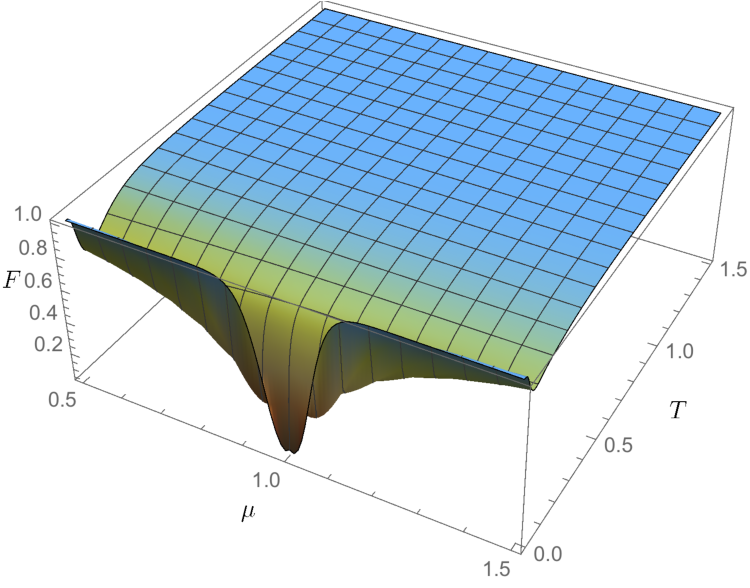
\includegraphics[width=0.7\textwidth,height=0.5\textwidth]{kitaev_fidelity_T.pdf}
\end{minipage}
\begin{minipage}{0.33\textwidth}
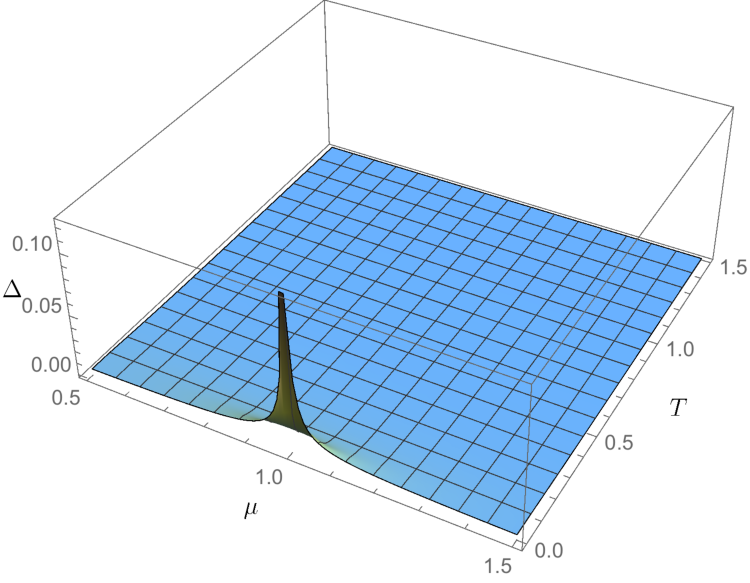
\includegraphics[width=0.7\textwidth,height=0.5\textwidth]{kitaev_uhlmann_theta.pdf}
\end{minipage}%
\caption{The fidelity for thermal states $\rho$, when probing the parameter of the Hamiltonian that drives the topological PT $\delta \mu =\mu'-\mu=0.01$ (left), and the temperature $\delta T=T'-T=0.01$ (centre), and the Uhlmann connection, when probing the parameter of the Hamiltonian $\mu$ (right), for the TSC Kitaev chain model. The plot for $\Delta$ when $\delta \mu=0$, is trivial (equal to zero everywhere), thus we omit it.}
\label{fig:fid:kit}
\end{figure}

For all the three cases that we presented the behaviour of the fidelity and the quantity $\Delta$ is qualitatively the same.
We see that for $T=0$ the fidelity exhibits a sudden drop in the neighbourhood of the gap-closing points, signalling the topological quantum PTs. As temperature increases, the drop of fidelity at the quantum critical points is rapidly smoothened towards the $F=1$ value. This shows the absence of both finite-temperature parameter-driven, as well as temperature-driven (i.e., thermal) PTs. The plots of $\Delta$ for $\delta T=0$, show a behaviour similar to that of the fidelity, while if we only change the temperature and not the parameter of the Hamiltonian, we obtain no information, as $\Delta$ is identically equal to zero, due to the triviality of the Uhlmann connection associated to the mutually commuting states (a consequence of the Hamiltonian's independence on the temperature). $\Delta$ is sensitive to PTs for which the state change is accompanied by a change of the eigenbasis (in contrast to fidelity, which is sensitive to both changes of eigenvalues and eigenvectors). For TIs and TSCs, this corresponds to parameter-driven transitions only. 
\section{Edge states of topological insulators and superconductors}
\label{sec:edge}
When one considers topological systems on a finite-size chain with open boundary conditions, the bulk-to-boundary correspondence principle~\cite{x:g:wen:91,ryu:hat:02} predicts the existence of zero modes localised at the ends of the chain, whenever the bulk is in a topologically non-trivial phase. It is then possible to consider the associated thermal states, $\rho=\exp(-\beta \mathcal{H})/Z$, and probe the effects of temperature. The study of the Uhlmann connection and the fidelity conducted in the previous section suggests that at zero temperature the edge states should exhibit an abrupt change as the system passes the point of quantum phase transition, while at finite temperatures they should smoothly change, slowly being washed away with the temperature increase, as a consequence of the absence of finite-temperature transitions. Below, we first study TIs in Section~\ref{sec:edgeTI}, while in Section~\ref{sec:edgeTSC} we analyse a TSC given by the Kitaev model, showing the agreement with the above inferred behaviour.

\subsection{Topological insulators}
\label{sec:edgeTI}
 Let us consider the Creutz ladder model as a representative of TIs. Similar results are obtained when considering the SSH model and we omit them for the sake of briefness. In the trivial phase, the spectrum decomposes into two bands of states separated by a gap. At zero chemical potential, the zero-temperature limit of $\rho$ is the projector onto the Fermi sea state $\ket{\text{FS}},$ obtained by occupying the lower band. On a topologically non-trivial phase, however, the spectrum is composed of the two bands {\em and} the zero modes. At zero chemical potential, the zero temperature limit of $\rho$ is now the projector onto the ground state manifold of $\mathcal{H}$, which is spanned by $\ket{\text{FS}}$ and additional linearly independent states by creating excitations associated to the zero modes. Since the Fermi sea does not have these edge state excitations (exponentially localised at the boundary) included, the occupation number as a function of position, $n_i=a_i^\dagger a_i+b_i^{\dagger}b_i$, will see this effect at the boundary of the chain. Indeed, this is what we see in Figure~\ref{fig:FS_occupation_number}: the occupation number, as a function of position, drops significantly at the edges in the topologically non-trivial phase. On the other hand, on the topologically trivial side the occupation number stays constant throughout the whole chain (both bulk and the edges).



\begin{figure}[h!]
\begin{minipage}{0.45\textwidth}
\centering
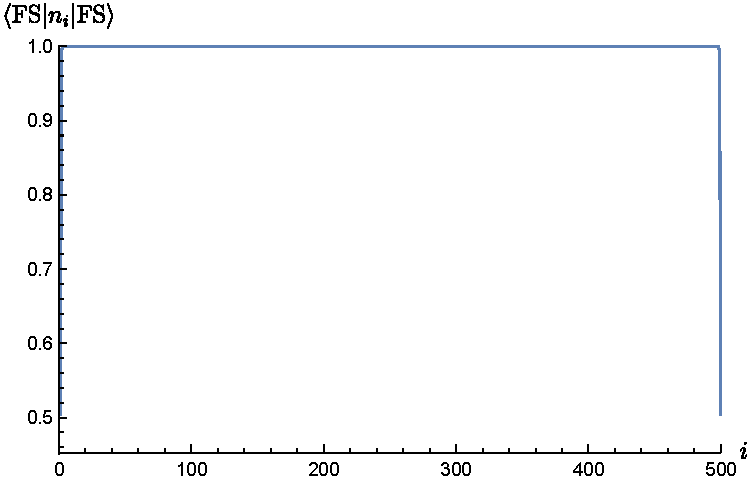
\includegraphics[scale=0.5]{fermisea_topological.pdf}
\end{minipage}
\begin{minipage}{0.45\textwidth}
\centering
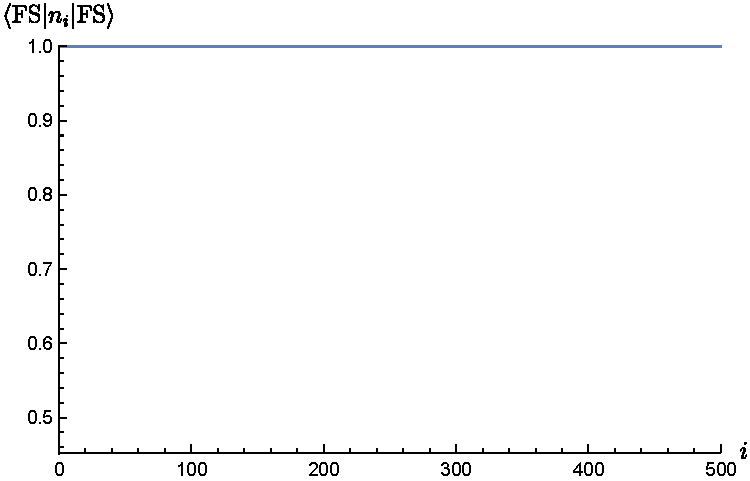
\includegraphics[scale=0.5]{fermisea_trivial.pdf}
\end{minipage}
\caption{Fermi sea expectation value of the occupation number $n_i=a_i^\dagger a_i+b_i^{\dagger}b_i$ as a function of position $i$ on a chain of 500 sites with open boundary conditions for a TI (Creutz ladder model). On the left panel the system is in a topologically non-trivial phase with $2K=1,M=0.1,\phi=\pi/2$. On the right panel the system is in a topologically trivial phase with $2K=1,M=1.0001,\phi=\pi/2$.}
\label{fig:FS_occupation_number}
\end{figure}



If we want the thermal state's $T=0$ limit to be the Fermi sea, we have to add a very small (negative) chemical potential. It has to be small enough so that the lower band gets completely filled. In the following Figure~\ref{fig:BG_occupation_number}, we see that the expectation value $\tr(\rho n_i)$ coincides with $\bra{\text{FS}}n_i\ket{\text{FS}}$ in the $T=0$ limit and the deviation of the occupation number at the edge from that in the bulk gets washed out smoothly as the temperature increases. In fact, in the large temperature limit, the state is totally mixed, implying that the expected value of the occupation number will be constant and equal to $1$, as a function of position.  

\begin{figure}[h!]
\begin{minipage}{0.45\textwidth}
\centering
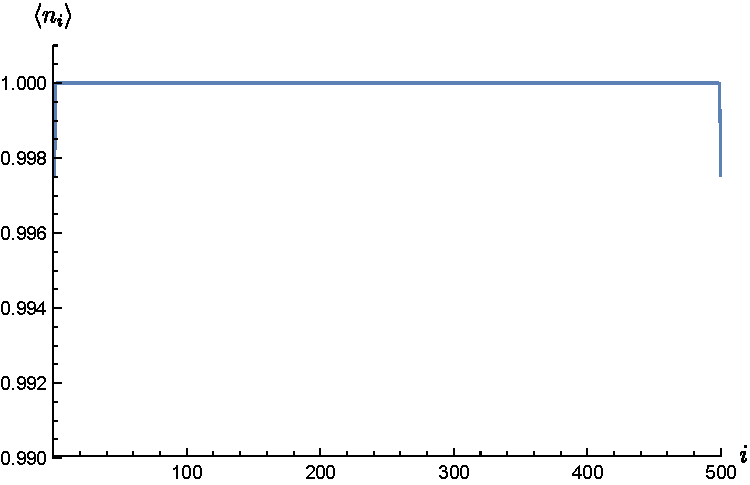
\includegraphics[scale=0.55]{occupation_T_100.pdf}
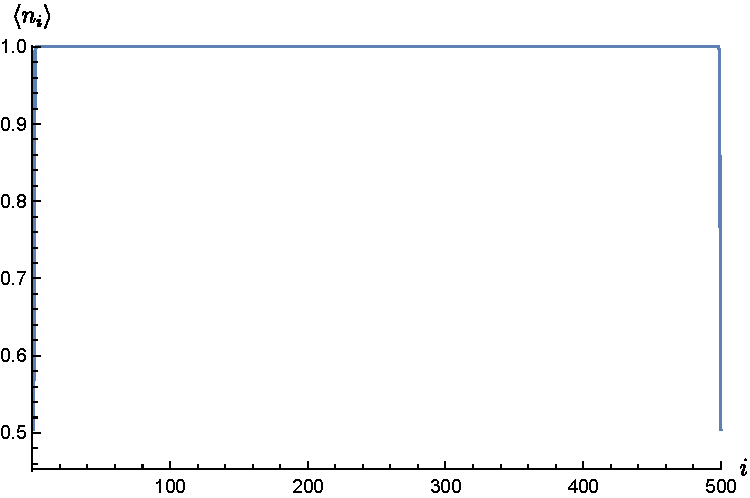
\includegraphics[scale=0.55]{occupation_zero_T.pdf}
\end{minipage}
\begin{minipage}{0.45\textwidth}
\centering
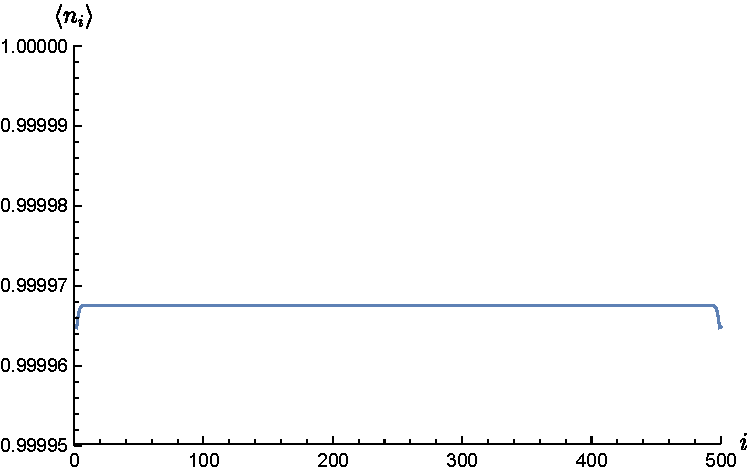
\includegraphics[scale=0.55]{occupation_finite_T_trivial.pdf}
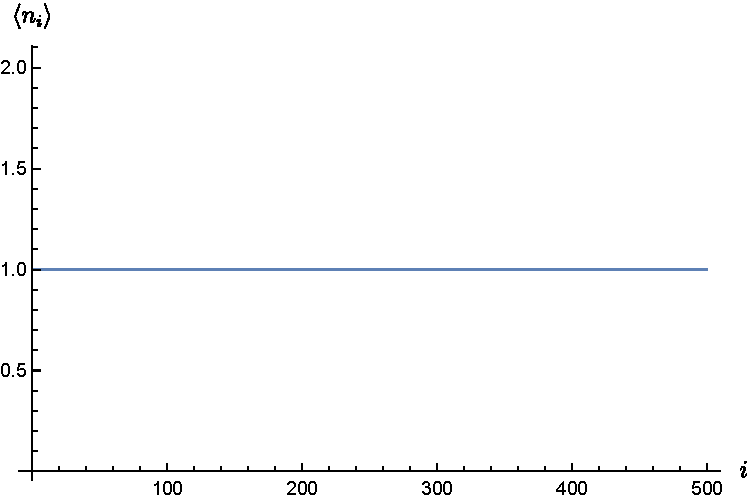
\includegraphics[scale=0.55]{occupation_zero_T_trivial.pdf}
\end{minipage}
\caption{Expectation value of the occupation number $n_i=a_i^\dagger a_i+b_i^{\dagger}b_i$ as a function of position $i$ on a chain of 500 sites with open boundary conditions for a TI (Creutz ladder model). In the left panel, we show the topologically non-trivial phase with $2K=1,M=0.1,\phi=\pi/2$, for temperatures $T=10^{-5}$ (down) and $T=0.2$ (up). On the right panel we have a topologically trivial phase near the critical value of the parameter $2K=1,M=1.0001,\phi=\pi/2$, for temperatures $T=10^{-5}$ (down) and $T=0.2$ (up). Increasing $M$, the edge behaviour is washed out smoothly, for finite $T$, and it becomes trivial as for the $T=0$ case.}
\label{fig:BG_occupation_number}
\end{figure}
We see that the results presented in Figures~\ref{fig:FS_occupation_number} and~\ref{fig:BG_occupation_number} confirm the results obtained by the fidelity analysis and the study of the Uhlmann connection in terms of the quantity $\Delta$. Indeed, the fact that the edge states localised at the boundary between two distinct topological phases, that manifest the topological order at zero temperature, are gradually smeared out as we increase the temperature, confirm the absence of finite-temperature PTs. Furthermore, our results on the edge states, obtained for systems in thermal equilibrium, agree with those concerning open systems treated within the Lindbladian approach~\cite{viy:riv:del:12} (and consequently, due to considerable computational hardness, obtained for an open chain of only 8 sites).

\subsection{Topological superconductors}
\label{sec:edgeTSC}
 As far as the TSC Kitaev model is concerned, the chemical potential is a parameter of the Hamiltonian and we cannot lift the zero modes from the zero-temperature limit of $\rho$ with the above method. Moreover, the Kitaev Hamiltonian does not conserve the particle number, and adding chemical potential associated to the total particle number would not lift the zero modes even if $\mu$ were not a parameter of the Hamiltonian.  Note though, that the total number of Bogoliubov {\em quasi-particles} which diagonalise the Hamiltonian is conserved. Hence, we add a very small (negative) chemical potential associated with the total quasi-particle number, thereby lifting the Majorana zero modes energy.  We found that the good quantity to be studied is not the occupation number as a function of the position in the chain, but the ratio between the average particle occupation number at the edge and the average particle occupation number at the bulk $f(\mu;T) = \langle n_{\text{edge}}\rangle/\langle n_{\text{bulk}}\rangle$ (without loss of generality, we have chosen for $n_{\text{bulk}}$ the site in the middle of the chain, since it is approximately constant throughout the bulk). 
 In Figure~\ref{fig:majorana}, we present the results obtained for a chain with open boundary conditions, consisting of 300 sites.
 
 
 \begin{figure}[h!]

\centering
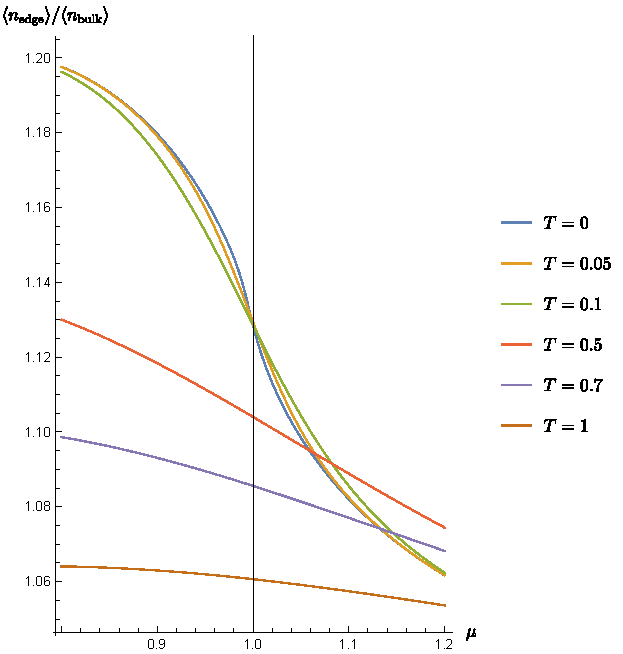
\includegraphics[scale=0.6]{majorana_paper_plot.pdf}

\caption{$\langle n_{\text{edge}}\rangle/\langle n_{\text{bulk}}\rangle$ as a function of the chemical potential $\mu$ for a chain of 300 sites with open boundary conditions, for several values of the temperature $T$.}
\label{fig:majorana}
\end{figure}

The results are consistent with the behaviour inferred by the Uhlmann connection and the fidelity: Majorana modes exhibit an abrupt change at zero temperature (a signature of the quantum PT), while for fixed finite temperatures they smoothly change with the parameter change, and are slowly washed away with the temperature increase. Indeed, the behaviour of the finite-temperature curves is smooth, while the zero-temperature quench-like curve is expected to develop a discontinuity at $\mu = 1$ in the thermodynamic limit (see for example Fig.4(b) and the respective discussion in~\cite{qua:zur:10}). To show this more accurately, one needs considerably higher computational power to probe chain lengths of much higher orders of magnitude, a relevant future direction of work. 

The behaviour of the edge states and the associated Majorana modes reveals an interesting property of these systems which, at finite temperatures, despite the absence of phase transitions, they keep exhibiting their topological features even on the ``trivial side'' of the phase diagram (for parameter values for which on zero temperature the system is topologically trivial). At zero temperature, the Majorana modes are known to be good candidates for qubit encoding, see~\cite{ali:12,ipp:riz:gio:maz:16,majorana:17,majorana:twist:17} and references therein. Therefore, the aforementioned property of Majorana modes at the low but finite-temperature regime, is potentially significant in constructing realistic quantum memories. Furthermore, the existence of stable quantum memories has considerable impact in cryptography~\cite{rod:mat:pau:sou:17,pir:ott:spe:wee:bra:llo:geh:jac:and:15,ber:chr:col:ren:ren:10,dam:feh:ren:sal:sch:07,weh:sch:ter:08,sch:ter:weh:09,ng:jos:che:kur:weh:12,koe:weh:wul:12,bou:feh:gon:sch:13,lou:alm:and:pin:mat:pau:14}, as explained in Chapter~1.

Finally, we should stress that this new method to study Majorana modes is more general and also applicable to TIs: since the Hamiltonian conserves the total particle number, and the quasi-particle creation operators are linear combinations of {\em just} the particle creation operators (and not of the holes as well), the total quasi-particle and particle numbers coincide in this case. The results obtained for TIs using this new method lead to the same qualitative conclusion regarding the behaviour of the edge states (consistent with our previous results) and we omit them in order to avoid repetition.


\section{Fidelity and $\Delta$ analysis of BCS superconductors}
\label{sec:bcs}
In this section we study a topologically trivial superconducting system, as described by the BCS theory~\cite{bar:coo:sch:57}, with the effective Hamiltonian 
\begin{eqnarray}
\label{eq:BCS_MF}
\mathcal{H}=\sum_{k} (\varepsilon_{k}-\mu)c_{k}^{\dagger}c_{k}-\Delta_{k} c_{k}^{\dagger}c_{-k}^{\dagger} + \text{H.c.},
\end{eqnarray}
where $\varepsilon_k$ is the energy spectrum, $\mu$ is the chemical potential, $\Delta_{k}$ is the superconducting gap, $c_{k}\equiv c_{k\uparrow}$ and $c_{-k}\equiv c_{-k \downarrow}$ are operators annihilating an electron with momentum $k$ and spin up and an electron with momentum $-k$ and spin down, respectively. The gap parameter is determined in the above mean-field Hamiltonian through a self-consistent mass gap equation and it depends on the original Hamiltonian's coupling associated to the lattice-mediated pairing interaction $V,$ absorbed in $\Delta_k$ (for more details, see~\cite{pau:vie:08}). The solution of the equation renders the gap temperature-dependent.
In Figure~\ref{fig:bcs}, we show the quantitative results for the fidelity and $\Delta$. 
\begin{figure}[h!]
\begin{minipage}{0.24\textwidth}
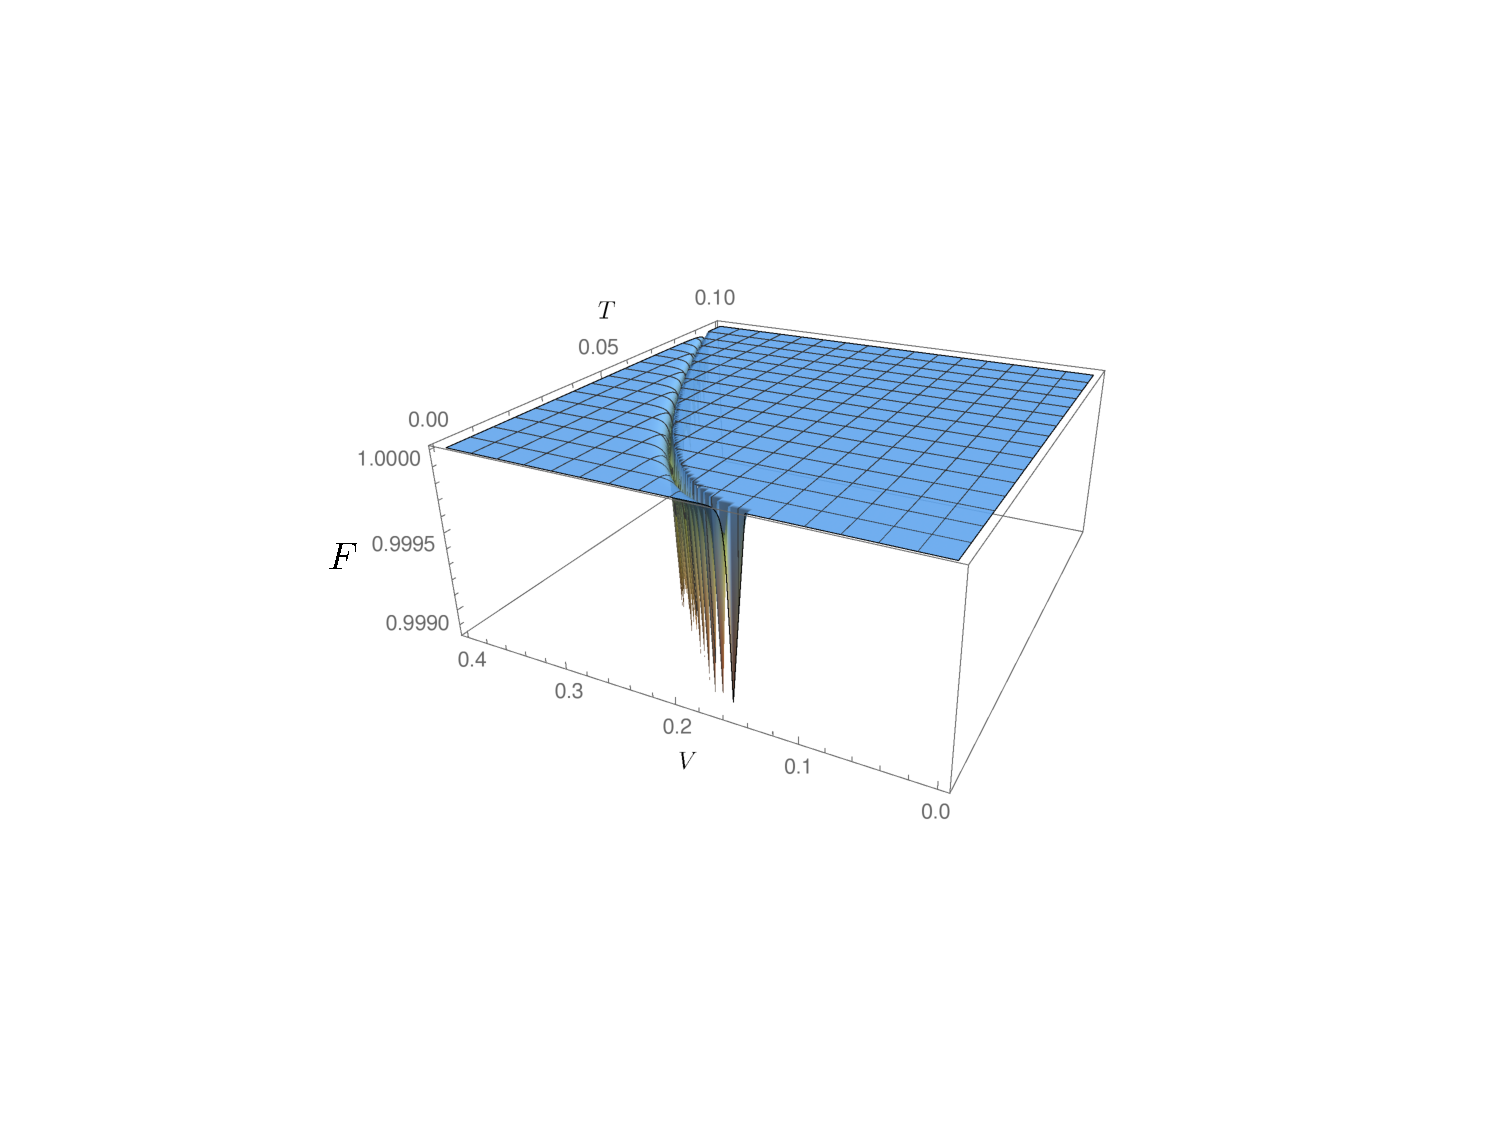
\includegraphics[width=0.8\textwidth,height=0.6\textwidth]{BCS_fidelity_theta.pdf}
\end{minipage}%
\begin{minipage}{0.24\textwidth}
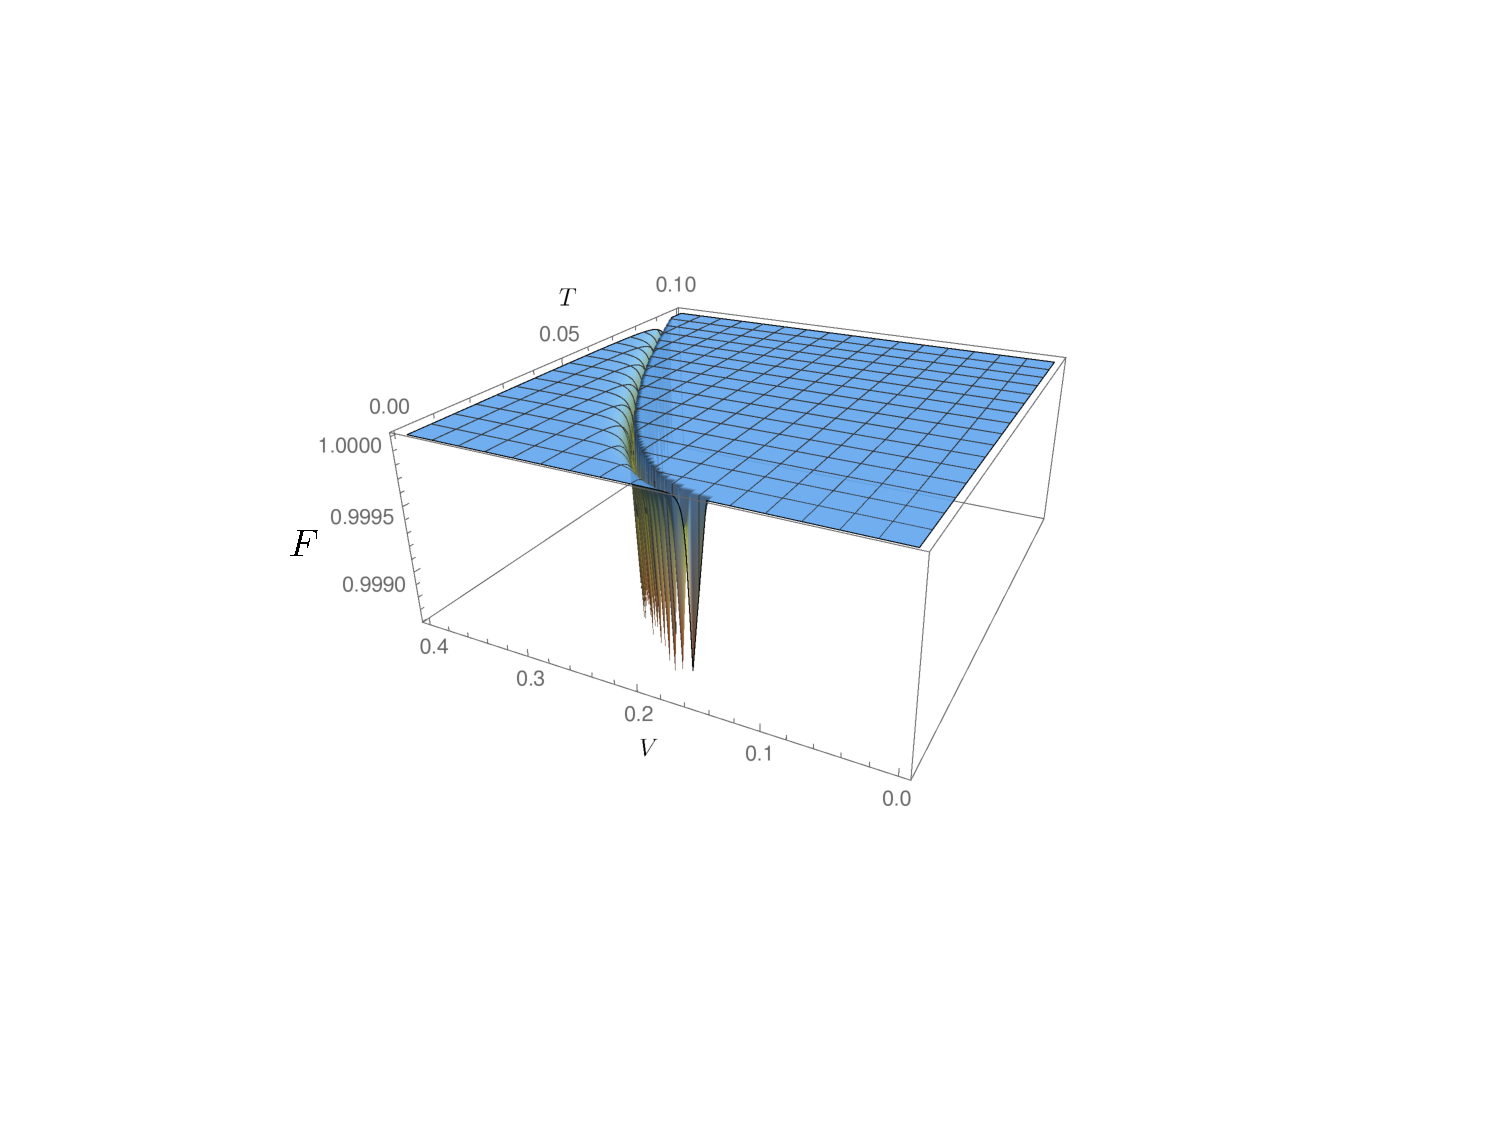
\includegraphics[width=0.8\textwidth,height=0.6\textwidth]{BCS_fidelity_T.pdf}
\end{minipage}
\begin{minipage}{0.24\textwidth}
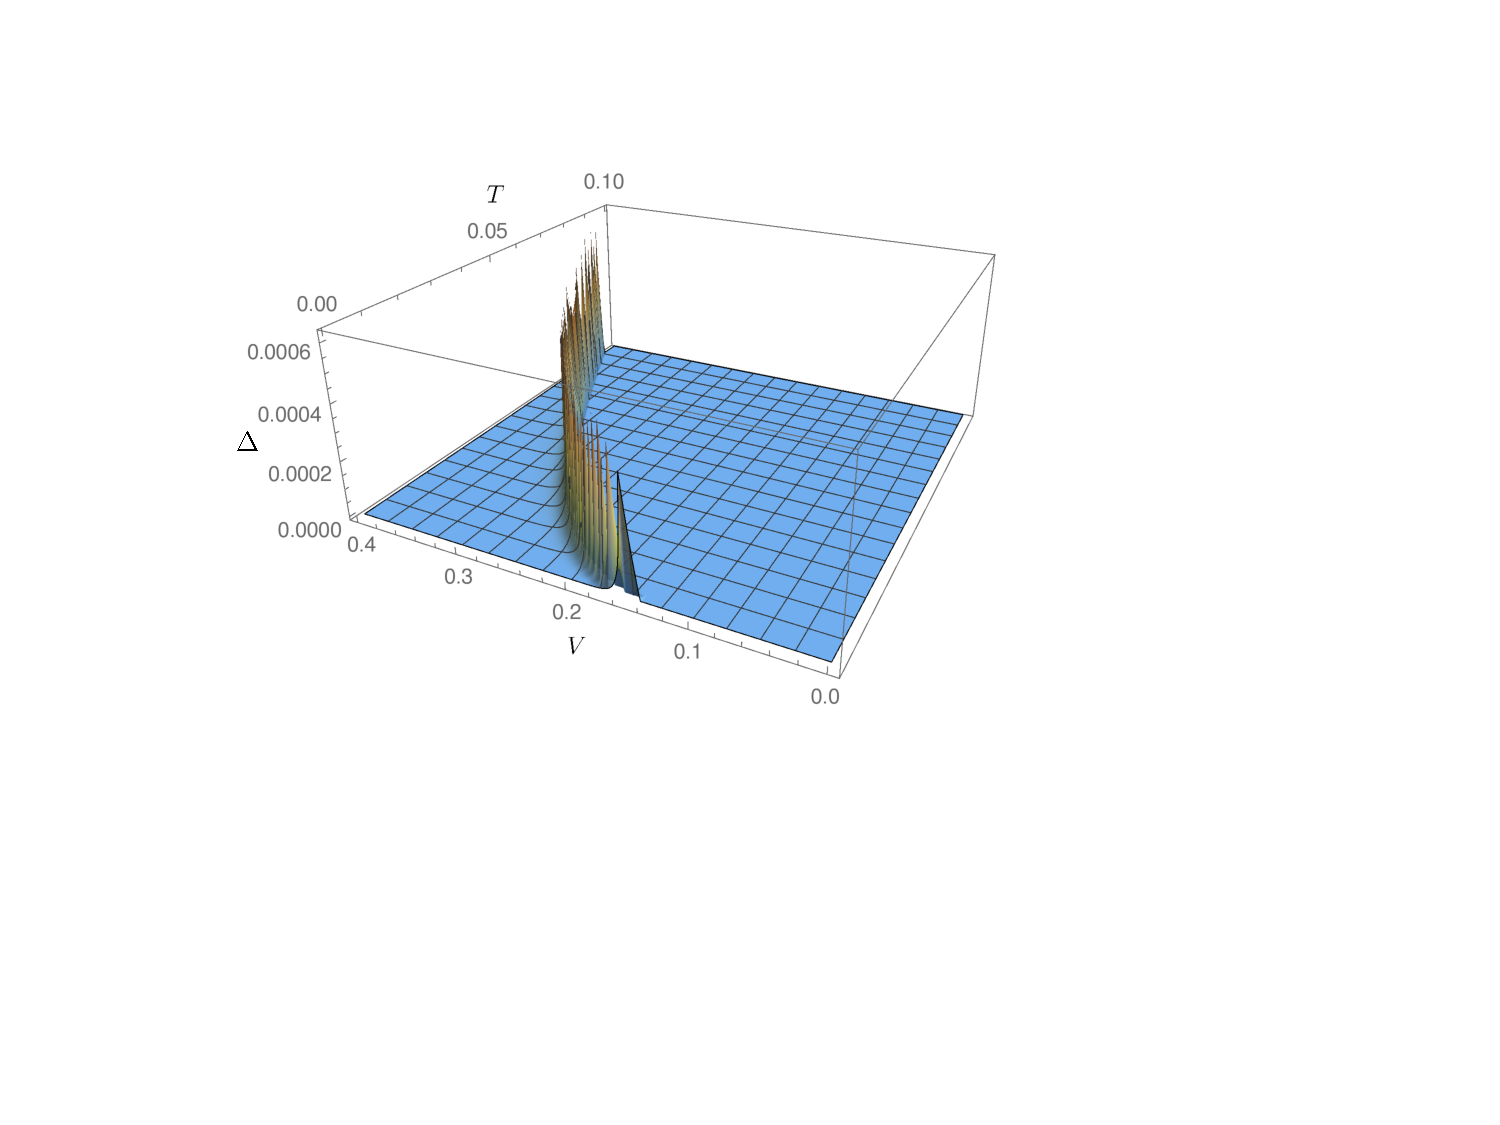
\includegraphics[width=0.8\textwidth,height=0.6\textwidth]{BCS_delta_theta.pdf}
\end{minipage}%
\begin{minipage}{0.24\textwidth}
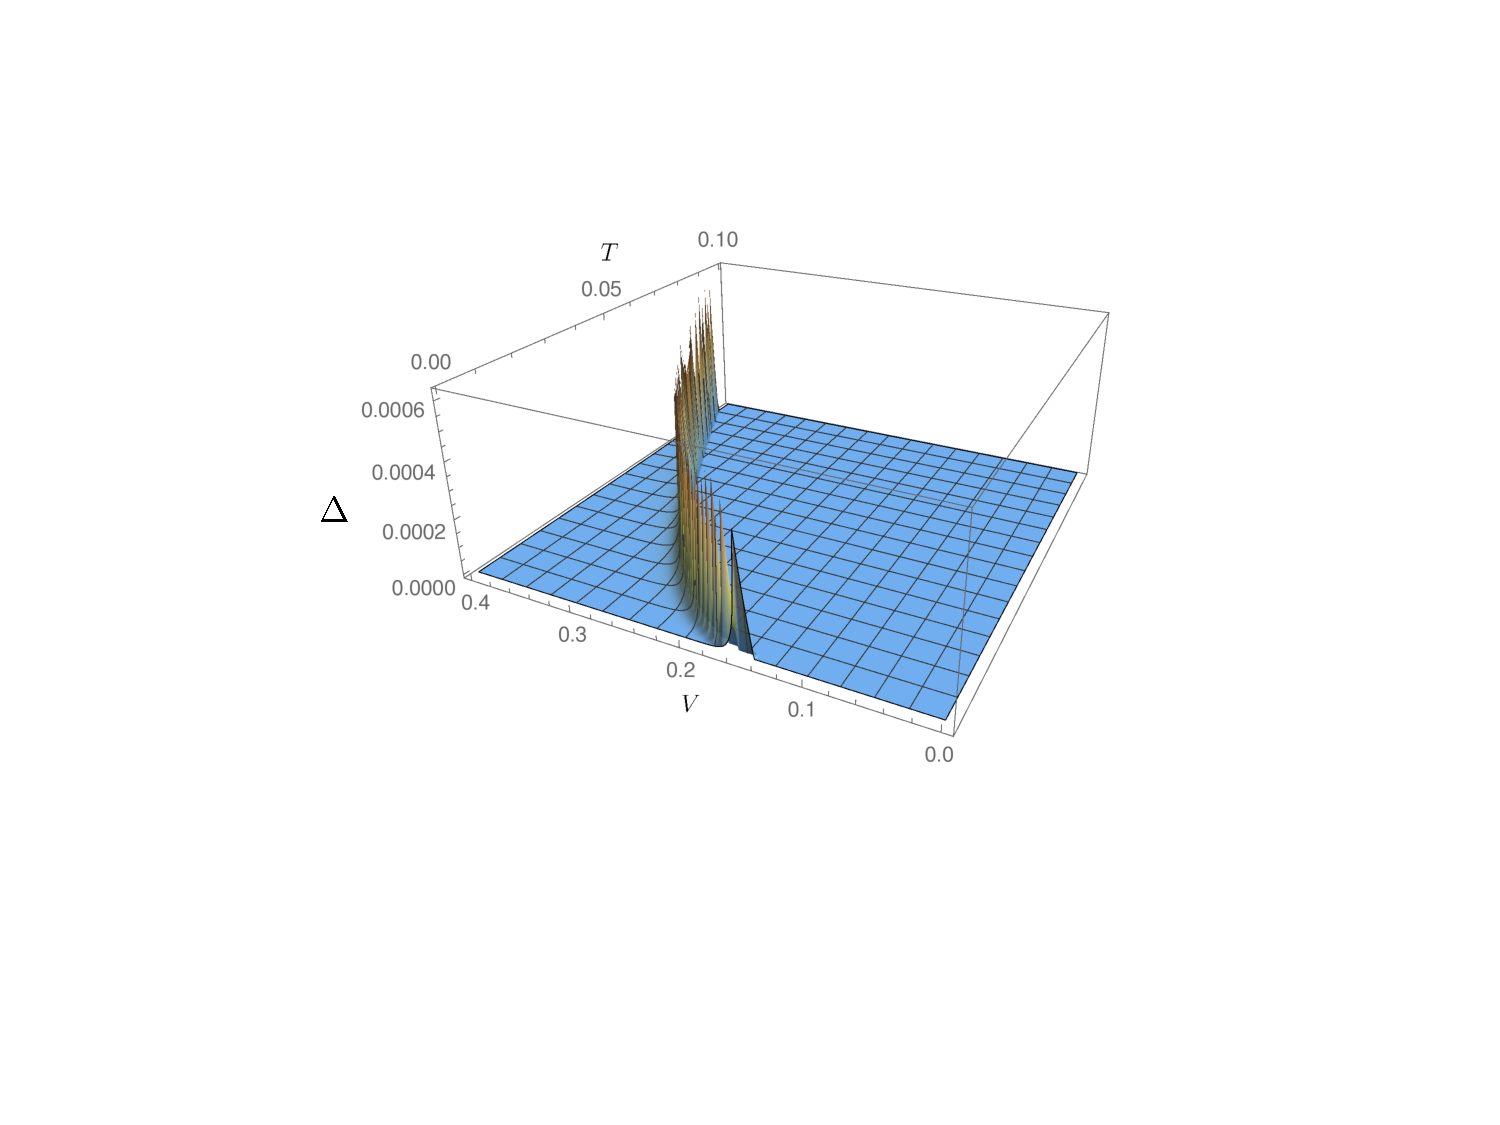
\includegraphics[width=0.8\textwidth,height=0.6\textwidth]{BCS_delta_T.pdf}
\end{minipage}
\caption{The fidelity for thermal states $\rho$ when probing the parameter of the Hamiltonian $\delta V =V'-V=10^{-3}$ (left) and the temperature $\delta T=T'-T=10^{-3}$ (centre left), and the Uhlmann connection (centre right and right, respectively), for BCS superconductivity.}
\label{fig:bcs}
\end{figure}
We observe that both quantities show the existence of thermally driven PTs, as their abrupt change in the point of criticality at $T=0$, survive and drift, as temperature increases. This behaviour is in sharp contrast to the respective behaviour of the topologically non-trivial systems, for which there exist no finite-temperature PTs.

It is interesting to compare the two cases of superconductors studied, and try to isolate the reasons for such difference. 
Unlike TSCs, in the BCS model the temperature does not only appear in the thermal state, but it is also a parameter of the effective Hamiltonian (recall that the superconducting gap depends on temperature), resulting in the change of the system's eigenbasis and consequently a non-trivial Uhlmann connection. In particular, the quantity $\Delta$, which quantifies the rate of change of the system's eigenbasis, reflects the quantum contribution to the state distinguishability (see also~\cite{zan:ven:gio:07}, equation (3), in which the Bures metric is split into classical and non-classical terms, the first quantifying the change of system's eigenvalues and the second the change of the corresponding eigenvectors). Thus, the Uhlmann connection is trivial in the cases of the topological systems considered, as their Hamiltonians do not explicitly depend on temperature and thus commute with each other at finite temperatures. On the other hand, the mean-field BCS Hamiltonian considered does explicitly depend on the temperature, and as the results presented above clearly show, the change of the eigenbasis of the BCS thermal states carries the signature of a thermally driven PT. Note that, having a purely non-classical contribution, such a temperature-driven PT has quantum features as well, which is on its own an interesting consequence of the study of the Uhlmann connection.

To illustrate this difference between TSCs and BCS better, let us explain the above with a few more details.
In the case of the BCS superconductivity we considered the effective mean-field Hamiltonian given by Equation~\eqref{eq:BCS_MF},
in which the gap $\Delta(V,T)$ is a function of temperature. Had we considered a more fundamental ``pairing Hamiltonian'', which takes into account the quartic electron interaction mediated by the phonons of the lattice,
\begin{equation}
\label{eq:BCS_P}
\mathcal{H}^{P}=\sum_{k} (\varepsilon_{k}-\mu)c_{k}^{\dagger}c_{k}-\sum_{k,k'} V_{k,k'}c_{k'}^{\dagger}c_{-k'}^{\dagger}c_{-k}c_{k} + \text{H.c.},	
\end{equation}
the Uhlmann connection would be trivial. The mean-field Hamiltonian of Equation~\eqref{eq:BCS_MF} is obtained from Equation~\eqref{eq:BCS_P} by means of the BCS decoupling scheme with an averaging procedure, setting the effective gap for the mean-field state $\rho = e^{-\beta\mathcal{H}}/Z$ (for simplicity, we assume $V_{kk'} = -V$ for $k,k'$ close to the Fermi momentum $k_F$, and zero otherwise) to be
\begin{equation}
\label{eq:gap}
\Delta(V,T) = -\sum_{k'} V_{kk'} \langle c_{-k}c_{k}\rangle = V \sum_k \mbox{Tr}(c_{-k}c_{k}\rho ).	
\end{equation}

In other words, the effective mean-field Hamiltonian of Equation~\eqref{eq:BCS_MF} is obtained from Equation~\eqref{eq:BCS_P} by expanding $c_{-k}c_{k} = \langle c_{-k}c_{k}\rangle + \delta(c_{-k}c_{k})$ around the suitably chosen superconducting ground state. Thus, $\mathcal{H}$ breaks the $\mbox{U}(1)-$~particle-number conservation symmetry of $\mathcal{H}^P$ to a residual $\mathbb Z_2$ symmetry, in order to accommodate the superconducting properties of the system. As a result, the Uhlmann connection becomes sensitive to temperature-driven PTs, due to the enhanced state distinguishability in terms of the system's eigenbasis. On the other hand, the Hamiltonian of the Kitaev model is phenomenological, modelled upon the success of the related BCS mean-field Hamiltonian. In this model, the gap is, for simplicity, considered to be temperature-independent. One might thus question whether the gap of a general superconducting material should also a priori depend on the temperature. It would be interesting to probe this  in experiments with realistic topological superconducting materials. Our method based on the Uhlmann connection could then be particularly useful in the analysis of such experiments.

\section{The choice of the parameter space in the study of topological phase transitions}
\label{sec:space}
We will conclude this chapter, by commenting on the relevance of the choice of the parameter space in the study of PTs in topologically ordered systems.
In order for the Uhlmann connection and the fidelity to be in tune, they must be taken over the same base space, which in our study consists of the parameters of the Hamiltonian and the temperature. In a previous study~\cite{viy:riv:del:14}, the Uhlmann connection for 1D topologically ordered systems was considered in the momentum space and with respect to single-particle density matrices of the form $\{\rho_k:=e^{-\beta H_k}/Z: k\in \mathcal B \}$. In order to infer the possibility of finite-temperature PTs, the authors used the Uhlmann geometric phase $\Phi_U(\gamma_c)$ along the closed curve $\gamma_c(k)=\rho_k$, given as 
\[
\Phi_U(\gamma_c)=\arg\tr\{w(-\pi)^{\dagger}w(\pi)\} =\arg\tr\{\rho_{\pi}U(\gamma_c)\},
\]
where $w(k)$ is the horizontal lift of the loop of density matrices $\rho_{k}$, and $U(\gamma_c)$ is the so-called Uhlmann holonomy obtained by imposing the Uhlmann parallel transport condition along the first Brillouin zone $\mathcal B$.
It was found that $\Phi_U(\gamma_c)$ changes abruptly from $\pi$ to $0$ after some ``critical'' temperature $T_U$. The authors identified this abrupt change of $\Phi_U(\gamma_c)$, as a finite-temperature topological PT ``in the Uhlmann sense'', in analogy to the pure-state case, where the abrupt change of the Berry phase signals a topological PT~\cite{ber:84}. Note, also, that the zero-temperature limit of the Uhlmann geometric phase is the Berry phase. However, for the topological systems studied in~\cite{viy:riv:del:14}, the Uhlmann holonomy is a smooth function of the temperature and is given, in the basis in which the CS operator is diagonal, by:
\label{eq:hol}
\[
U(\gamma_c) = \exp \Big\{-\frac{i}{2} \int_{-\pi}^{\pi} \left[1 - \text{sech} \left(\frac{E_k}{2T}\right)\right]\frac{\partial \varphi_k}{\partial k}dk\  \sigma_z\Big\},
\]
where $\varphi_k$ is the polar angle coordinate of the vector $\vec{n}_k$ lying on the equator of the Bloch sphere.  So, while the Uhlmann phase suffers from an abrupt change, the Uhlmann holonomy is smooth, hence there is no PT-like behaviour. Conversely, there might be cases, where the Uhlmann phase is trivial, $\Phi_U(\gamma_c) = 0$, while the corresponding holonomy is not, $U(\gamma_c)\neq I$.
Moreover, the associated critical temperature is not necessarily related to a physical quantity that characterises a system's phase.\\

In the paradigmatic case of the quantum Hall effect~\cite{and:mat:uem:75}, at $T=0$, the Hall conductivity is quantised in multiples of the first Chern number of a vector bundle in momentum space through several methods. For example, one can use linear response theory or integrate the fermions to obtain the effective action of an external $\text{U}(1)-$~gauge field. The band topology appears, thus, in the response of the system to an external field. In this context, it is unclear how the Uhlmann geometric phase along the cycle of the 1D momentum space, can have an interpretation in terms of the physical response of the system. In order to measure it, one would have to be able to change the quasi-momentum of a state in an adiabatic way. In realistic setups, the states at finite temperatures are statistical mixtures over all momenta, such as the thermal states considered, and realising closed curves of states $\rho_k$ with precise momenta changing in an adiabatic way seems to be a tricky task. The fidelity computed in our work though, refers to the change of the system's {\em overall} state, with respect to its parameters (controlled in the laboratory much like an external gauge field), and is related to an, \textit{a priori}, physically relevant geometric quantity, the Uhlmann factor $V$. The quantity $\Delta$, which can  be written as $\Delta=\tr \big[|\sqrt{\rho(t+\delta t)}\sqrt{\rho(t)}|(I-V)\big]$ also contains information about the Uhlmann factor, therefore it seems that both of these quantities, computed over the base space consisting of the parameters of the Hamiltonian and the temperature, are physically more sensible to be considered in order to infer the possibility of PTs.


\section*{Conclusions and future work}
\label{Conclusions and Outlook}

By means of the fidelity and the Uhlmann connection analysis, we showed the absence of finite-temperature PTs in 1D TIs and TSCs. We further confirmed this result through the study of the edge states that appear on the boundary between two distinct topological phases. We also performed the same analysis for a topologically trivial BCS superconductor, where, in contrast to the former systems, temperature-driven PTs occur and are captured by both the fidelity and the Uhlmann connection. This shows that, when changing the temperature, the density operator is changing both at the level of its spectrum and its eigenvectors. We analysed in detail the origin of the differences between topologically trivial and non-trivial superconductors and suggested that, in realistic scenarios, the gap of TSCs could also, generically, be temperature-dependent. We also discussed the relevance of the choice of the base space. We clarified that the Uhlmann geometric phase considered in \textit{momentum space} is not adequate to infer such PTs, since it is only a part of the information contained in the Uhlmann holonomy. Indeed, this holonomy, as a function of temperature, is smooth (Equation~\eqref{eq:hol}), hence no PT-like phenomenon is expected.

  Finally, we would like to point out possible future lines of research. The study of Majorana modes at finite temperature suggested that they can be used in achieving realistic quantum memories. The detailed quantitative analysis of their robustness, in concrete practical implementations, is a relevant direction for future work. Another related subject is to perform the same fidelity and Uhlmann connection analysis in the context of open systems, where the system interacts with a bath and eventually thermalises. There, the parameter space would also include the parameters associated to the system-bath interaction.


%
%
%
%\bibliography{bibforthesis}
%\bibliographystyle{unsrt}
%
%\end{document}
